\documentclass[11pt]{article}

% all packages used by any paper must be listed here
\usepackage{newsdebulletin,times,subcaption,epsfig,wrapfig,algorithmic,color,boxedminipage,graphicx,url}

\usepackage{etoolbox, totcount}
\usepackage{import}


% \usepackage{makecell}
% \usepackage{multirow}
% \usepackage{booktabs}
% \usepackage{amsfonts}
% \usepackage{amsmath,epsfig}
% \usepackage{graphicx}

% \usepackage{balance}
% \usepackage{xspace,colortbl,multirow}
% \usepackage{mathrsfs}
% \usepackage{amsmath}
% \usepackage{cancel}
% \usepackage{array}
% \usepackage{verbatim}
% \usepackage{bbm}
% \usepackage{bm}
% \usepackage{amsfonts}
% \usepackage{color}
% \usepackage{eurosym}
% \usepackage{setspace,lipsum}
% \usepackage{amsmath,amsfonts}
% \usepackage{authblk}

% \usepackage{url}
% \usepackage{multirow}
% \usepackage{paralist}
% \usepackage{mathtools}
% \usepackage{listings}
% \usepackage{soul}
% \usepackage{enumitem}
% \usepackage{fancyvrb}

% Break URLs properly
\def\UrlBreaks{\do-\do\.\do\@\do\\\do\!\do\_\do\|\do\;\do\>\do\]\do\)\do\,\do\?\do\'\do+\do\=\do\#}
\def\UrlBigBreaks{\do\:\do\/}




%\usepackage{algorithm,algorithmicx,algpseudocode}

%\usepackage[font=small,labelfont=bf]{caption}


\begin{document}

% you may want to put in real date, vol no, issue no- but that is not necessary
\bulletindate{June 2020}
\bulletinvolume{41}
\bulletinnumber{2}
\bulletinyear{2020}

% these are files that I have- but your part of the issue can be done without
% them
\IEEElogo{cs.pdf}
\insidefrontcover{incvA18.pdf}
% \insidebackcover[TCDE Membership Form]{./calls/joinTCDE16.ps}

\begin{bulletin}

%
%  Letters to the editor section.  Use the lettersection environment.
%  Each letter is contained in a letter environment, where the two required
%  options to \begin{letter} are the author and the address of the author.
%

\begin{lettersection}

% there will be other letters- and a blank page will appear in your document
% but the special issue part will be fine

\begin{letter}{Letter from the Editor-in-Chief}
{David Lomet}{Microsoft Corporation}
\documentclass[11pt]{article} 

\usepackage{deauthor,times,graphicx}
%\usepackage{url}
\usepackage{hyperref}

\begin{document}

\subsection*{ICDE 2018}

Repeating my comment from the last issue-

The IEEE International Conference on Data Engineering will be held in April 14-19, 2018 in Paris, France.  This is the flagship conference of the Computer Society's Technical Committee on Data Engineering.  It is a great conference, at a great location.  What could possibly be better than April in Paris at ICDE!  I am attending and hope to see you there.

\subsection*{About the Bulletin}

This March current issue marks the end of editorial tenure for the Bulletin's current set of editors.  So it is once again time for me to pat myself on the back.  This current set, Tim Kraska, Tova Milo, and Haixun Wang, continue my outstanding success (he says modestly) in finding and choosing great editors.  All three have done truly fine jobs at producing issues that bring to our readers surveys of the latest work in very current areas. The success of the Bulletin depends on great issue editors.  I want to thank Tim, Tova, and Haixun for being exactly that with the fine jobs that they have done.  There was unexpected ``scrambling" over the past two years, so I want to thank them also for their flexibility in coping with this.  


\subsection*{The Current Issue}

Don't you get tired of someone shouting ``FAKE NEWS!".  Or perhaps even worse, being exposed to fake news before it has been labeled as such?  Our political conversations seem increasingly to include many variations of ``fake news" and discussions about which news is fake.  ``Sad." So where am I going with this?

The database world has been working on a key aspect of this problem for many years.  The technical area is called ``data provenance".  And it addresses the problem of where information comes from and how it impacts the subsequent processing of data and the reported results.  The June, 2010 issue was the last one on provenance.  And seven years is a long time in an active technical area, especially an area as important as this.

The current issue is focused on the applications of provenance.  Without delving into the current political scene, a reader will clearly see how extensively provenance management can be used.  As we gain more insight into its application scenarios, we also gain more insight into how to manage provenance.  This symbiotic relationship is driving the field forward.   Tova Milo, our Bulletin editor for the issue, has done an excellent job in bringing the issue together, making it a great place to learn about and track progress in the field.  The result is an issue well worth reading.



\end{document}



\end{letter}
%
\newpage
%
%% your introductory letter goes here
%

\begin{letter}{Letter from the Special Issue Editor}
{Joseph E. Gonzalez}{University of California at Berkeley\\ Berkeley, CA}
\graphicspath{{letters/}}
\documentclass[11pt]{article} 

\usepackage{deauthor,times,graphicx}
%\usepackage{url}
\usepackage{hyperref}



\begin{document}

Machine learning is rapidly maturing into an engineering discipline at the center of a growing range of applications.
This widespread adoption of machine learning techniques presents new challenges around the management of the data, code, models, and their relationship throughout the machine learning life-cycle.
In this special issue, 
% of the Data Engineering Bulletin 
we have solicited work from both academic and industrial leaders 
% in the data engineering community that 
who are exploring how data engineering techniques can be used to address the challenges of the machine learning life-cycle.




\begin{figure}[h]
\centering
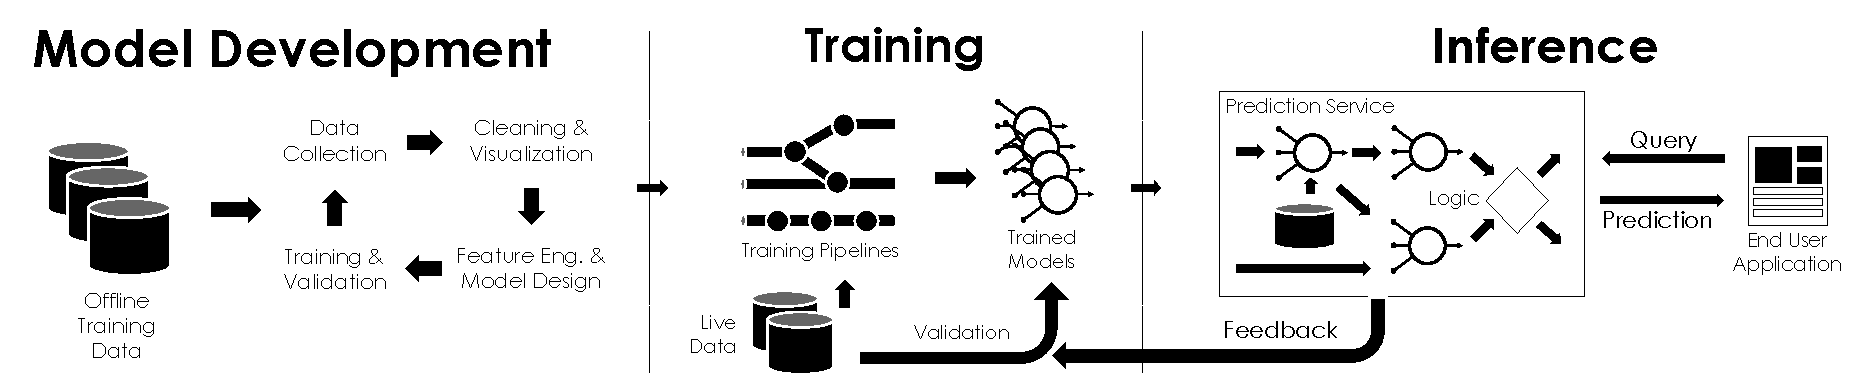
\includegraphics[width=\textwidth]{letters/pipeline.pdf}
\caption{\small \textbf{Machine Learning Life-cycle.} A simplified depiction of the key stages of a machine learning application.}
\label{fig:mllc}
\end{figure}


The machine learning life-cycle (Fig.~\ref{fig:mllc}) spans not only the model development but also production training and inference.
Each stage demands different skills (e.g., neural network design, data management, and cluster management) and imposes different requirements on the underlying systems.
Yet there is an overwhelming need for unifying design principles and technologies to address pervasive problems including feature management, data provenance, pipeline reproducibility, low-latency serving, and prediction monitoring just to name a few.


There has been a flurry of recent progress in systems to aid in managing the machine learning life-cycle.  
Large industrial projects like 
FB Learner Flow 
% \href{https://code.fb.com/core-data/introducing-fblearner-flow-facebook-s-ai-backbone/}{FB Learner Flow}
from Facebook, 
Michelangelo 
% \href{https://eng.uber.com/michelangelo/}{Michelangelo} 
from Uber, and 
TFX 
% \href{https://www.tensorflow.org/tfx/}{TFX} 
from Google have received considerable recent attention.  
In this issue, we have solicited papers from several recent industrial and academic projects that have received slightly less attention.


The first paper provides an overview of several real-world use cases and then outlines the key conceptual, data management, and engineering challenges faced in production machine learning systems.
% Rather than advocating a single system, this work describes some design principles that can inform potential solutions.
The second and third papers explores the challenges of model management and provenance across the machine learning life-cycle.
They motivate the need for systems to track models and their meta-data to improve reproducibility, collaboration, and governance. 
% expands upon the machine learning life-cycle 
% to include: data preparation, feature engineering, model training, deployment, and maintenance
% and explores the challenges of model 
The second paper introduces, ModelDB, an open-source system for model management and describe some of the functionality and design decisions. 
The third paper describes a related system, ProvDB, that uses a graph data model to capture and query fine-grained versioned lineage of data, scripts, and artifacts throughout the data analysis process.
The fourth paper describes, MLFlow, a new open-source system to address the challenges of experimentation, reproducibility, and deployment. 
This work leverages containerization to capture the model development environment and a simple tracking API to enable experiment tracking.
% The extensible model containerization enables model developers to more easily collaborate around modeling environments and then deploy model containers.
The fifth paper focuses on inference and explores the challenges and opportunities of serving white-box prediction pipelines.  
Finally, we solicited a summary of the recent Common Modeling Infrastructure (CMI) workshop at KDD 2018, which provides a summary of the keynotes and contributed talks.

The work covered here is only a small sample of the emerging space of machine learning life-cycle management systems. 
We anticipate that this will be a growing area of interest for the data engineering community.


% In contrast to the containerization of pipelines in MLFlow, the Microsoft team leverage knowledge about the internal of the prediction pipeline to more efficient serve predictions. 



\end{document}



\end{letter}

\end{lettersection}



% put the name of your special issue below
\begin{articlesection}{Data Technologies Behind Digital Contact Tracing for COVID19}
%
%  Contributed articles section.  Use the articlesection environment.
%  Each article is contained in an article environment, where the two required
%  options to \begin{article} are the title and author of the article
%
%\begin{article}
%{Title of article}
%{list of authors}
%\input{author-name/article.tex}
%\end{article}


\begin{article}
{Contact Tracing: Holistic Solution Beyond Bluetooth}
{Ramesh Raskar, Deepti Pahwa, Robson Beaudry }
% \def\input@path{{{submissions/BerkeleyCovista/}{submissions/BerkeleyCovista/}}}
\graphicspath{{submissions/safepaths/}}
\subimport{submissions/safepaths/}{safepaths.tex}
\end{article}


\begin{article}
{Slowing the Spread of Infectious Diseases Using Crowdsourced Data}
{Sydney Von Arx, Isaiah Becker-Mayer, Daniel Blank, Jesse Colligan, Rhys Fenwick, Mike Hittle, Mark Ingle, Oliver Nash, Victoria Nguyen, James Petrie, Jeff Schwaber, Zsombor Szabo, Akhil Veeraghanta, Mikhail Voloshin, Tina White, Helen Xue}
% \def\input@path{{{submissions/BerkeleyCovista/}{submissions/BerkeleyCovista/}}}
\graphicspath{{submissions/covidwatch/}}
\subimport{submissions/covidwatch/}{covidwatch.tex}
\end{article}


\begin{article}
{CoVista: A Unified View on Privacy Sensitive Mobile Contact Tracing Effort}
{David Culler, Prabal Dutta, Gabe Fierro, Joseph E. Gonzalez, Nathan Pemberton, Johann Schleier-Smith, K. Shankari, Alvin Wan, Thomas Zachariah}
% \def\input@path{{{submissions/BerkeleyCovista/}{submissions/BerkeleyCovista/}}}
\graphicspath{{submissions/BerkeleyCovista/figs/}}
\subimport{submissions/BerkeleyCovista/}{ms.tex}
\end{article}


\end{articlesection}

% \begin{newssection}{TCDE Election}

% % % there will be other letters- and a blank page will appear in your document
% % % but the special issue part will be fine

% % \begin{news}{Letter from the Editor-in-Chief}
% % {David Lomet}{Microsoft Corporation}
% % \documentclass[11pt]{article} 

\usepackage{deauthor,times,graphicx}
%\usepackage{url}
\usepackage{hyperref}

\begin{document}

\subsection*{ICDE 2018}

Repeating my comment from the last issue-

The IEEE International Conference on Data Engineering will be held in April 14-19, 2018 in Paris, France.  This is the flagship conference of the Computer Society's Technical Committee on Data Engineering.  It is a great conference, at a great location.  What could possibly be better than April in Paris at ICDE!  I am attending and hope to see you there.

\subsection*{About the Bulletin}

This March current issue marks the end of editorial tenure for the Bulletin's current set of editors.  So it is once again time for me to pat myself on the back.  This current set, Tim Kraska, Tova Milo, and Haixun Wang, continue my outstanding success (he says modestly) in finding and choosing great editors.  All three have done truly fine jobs at producing issues that bring to our readers surveys of the latest work in very current areas. The success of the Bulletin depends on great issue editors.  I want to thank Tim, Tova, and Haixun for being exactly that with the fine jobs that they have done.  There was unexpected ``scrambling" over the past two years, so I want to thank them also for their flexibility in coping with this.  


\subsection*{The Current Issue}

Don't you get tired of someone shouting ``FAKE NEWS!".  Or perhaps even worse, being exposed to fake news before it has been labeled as such?  Our political conversations seem increasingly to include many variations of ``fake news" and discussions about which news is fake.  ``Sad." So where am I going with this?

The database world has been working on a key aspect of this problem for many years.  The technical area is called ``data provenance".  And it addresses the problem of where information comes from and how it impacts the subsequent processing of data and the reported results.  The June, 2010 issue was the last one on provenance.  And seven years is a long time in an active technical area, especially an area as important as this.

The current issue is focused on the applications of provenance.  Without delving into the current political scene, a reader will clearly see how extensively provenance management can be used.  As we gain more insight into its application scenarios, we also gain more insight into how to manage provenance.  This symbiotic relationship is driving the field forward.   Tova Milo, our Bulletin editor for the issue, has done an excellent job in bringing the issue together, making it a great place to learn about and track progress in the field.  The result is an issue well worth reading.



\end{document}



% % \end{news}
% % %
% % \newpage
% % %
% % %% your introductory letter goes here
% % %
% % \begin{news}{Letter from the Special Issue Editor}
% % {Joseph E. Gonzalez}{University of California at Berkeley\\ Berkeley, CA}
% % \graphicspath{{letters/}}
% % \documentclass[11pt]{article} 

\usepackage{deauthor,times,graphicx}
%\usepackage{url}
\usepackage{hyperref}



\begin{document}

Machine learning is rapidly maturing into an engineering discipline at the center of a growing range of applications.
This widespread adoption of machine learning techniques presents new challenges around the management of the data, code, models, and their relationship throughout the machine learning life-cycle.
In this special issue, 
% of the Data Engineering Bulletin 
we have solicited work from both academic and industrial leaders 
% in the data engineering community that 
who are exploring how data engineering techniques can be used to address the challenges of the machine learning life-cycle.




\begin{figure}[h]
\centering
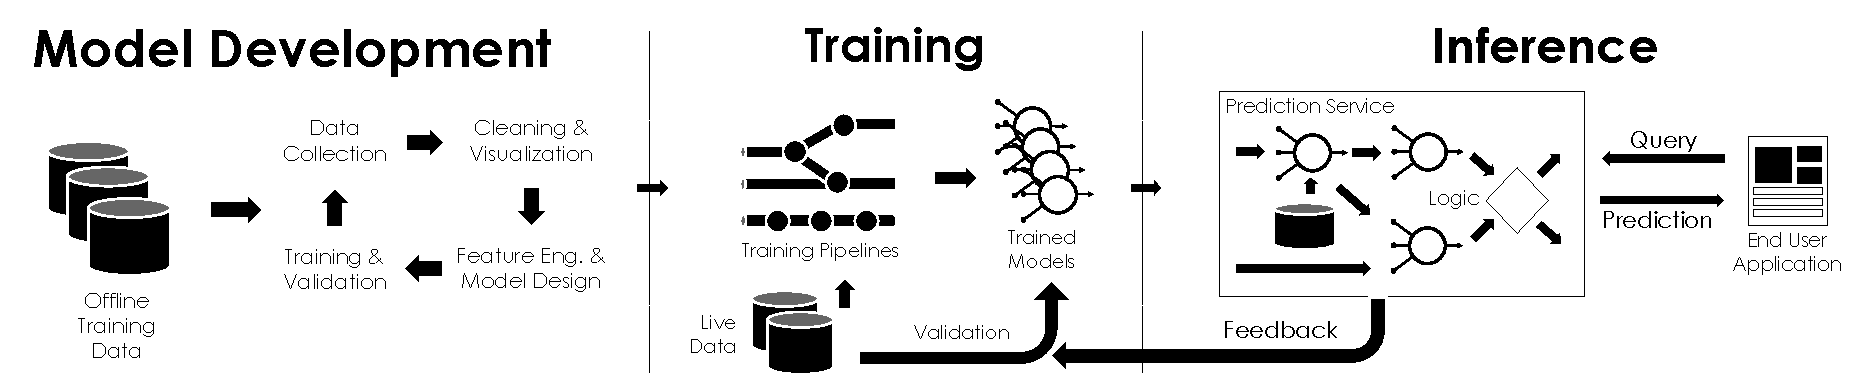
\includegraphics[width=\textwidth]{letters/pipeline.pdf}
\caption{\small \textbf{Machine Learning Life-cycle.} A simplified depiction of the key stages of a machine learning application.}
\label{fig:mllc}
\end{figure}


The machine learning life-cycle (Fig.~\ref{fig:mllc}) spans not only the model development but also production training and inference.
Each stage demands different skills (e.g., neural network design, data management, and cluster management) and imposes different requirements on the underlying systems.
Yet there is an overwhelming need for unifying design principles and technologies to address pervasive problems including feature management, data provenance, pipeline reproducibility, low-latency serving, and prediction monitoring just to name a few.


There has been a flurry of recent progress in systems to aid in managing the machine learning life-cycle.  
Large industrial projects like 
FB Learner Flow 
% \href{https://code.fb.com/core-data/introducing-fblearner-flow-facebook-s-ai-backbone/}{FB Learner Flow}
from Facebook, 
Michelangelo 
% \href{https://eng.uber.com/michelangelo/}{Michelangelo} 
from Uber, and 
TFX 
% \href{https://www.tensorflow.org/tfx/}{TFX} 
from Google have received considerable recent attention.  
In this issue, we have solicited papers from several recent industrial and academic projects that have received slightly less attention.


The first paper provides an overview of several real-world use cases and then outlines the key conceptual, data management, and engineering challenges faced in production machine learning systems.
% Rather than advocating a single system, this work describes some design principles that can inform potential solutions.
The second and third papers explores the challenges of model management and provenance across the machine learning life-cycle.
They motivate the need for systems to track models and their meta-data to improve reproducibility, collaboration, and governance. 
% expands upon the machine learning life-cycle 
% to include: data preparation, feature engineering, model training, deployment, and maintenance
% and explores the challenges of model 
The second paper introduces, ModelDB, an open-source system for model management and describe some of the functionality and design decisions. 
The third paper describes a related system, ProvDB, that uses a graph data model to capture and query fine-grained versioned lineage of data, scripts, and artifacts throughout the data analysis process.
The fourth paper describes, MLFlow, a new open-source system to address the challenges of experimentation, reproducibility, and deployment. 
This work leverages containerization to capture the model development environment and a simple tracking API to enable experiment tracking.
% The extensible model containerization enables model developers to more easily collaborate around modeling environments and then deploy model containers.
The fifth paper focuses on inference and explores the challenges and opportunities of serving white-box prediction pipelines.  
Finally, we solicited a summary of the recent Common Modeling Infrastructure (CMI) workshop at KDD 2018, which provides a summary of the keynotes and contributed talks.

The work covered here is only a small sample of the emerging space of machine learning life-cycle management systems. 
We anticipate that this will be a growing area of interest for the data engineering community.


% In contrast to the containerization of pipelines in MLFlow, the Microsoft team leverage knowledge about the internal of the prediction pipeline to more efficient serve predictions. 



\end{document}



% % \end{news}


% \end{newssection}



\begin{callsection}
%  This section will be empty for your version
%
%  Calls for papers section.  Use the callsection environment.
%  Each call for papers is contained in an call environment, where the single
%  required options to \begin{call} is the name of the conference.
%
\begin{call}{ICDE 2019 Conference}
%\centerline{\includegraphics[width=\textwidth, bb= 0 0 610 790]
% \centerline{
\includegraphics[width=\textwidth, bb= 0 0 590 760] {calls/icde19.pdf}}
\end{call}
\end{callsection}

\end{bulletin}
\end{document}
